\section{Model description} \label{Model-description}
\subsection{Reactor design}

The Chinese Academy of Sciences started the program of Thorium Molten Salt Reactor (TMSR) in 2011 \cite{jiang2012advanced}, and many works have been done on the design of MSR and the use of Thorium with the Th-U fuel cycle \cite{li2015analysis}. Among them, the SD-TMSR is proposed in 2018 \cite{li_optimization_2018}, which is a graphite-moderated molten salt reactor with thermal power of 2,250 MW$_{th}$. The design of the SD-TMSR is inspired by the \gls{MSBR} \cite{robertson_conceptual_1971} and the \gls{TMSR} \cite{nuttin2005potential}, which combines the advantages of high breeding ratio (BR) in fast spectrum and low fissile inventory of $^{233}$U in thermal spectrum. SD-TMSR also offers a negative and strong temperature coefficient of reactivity \cite{li_optimization_2018}. Figure~\ref{fig:ff} illustrates the quarter-core view of the
SD-TMSR. The core of the 
SD-TMSR is a right cylinder divided into an inner zone (486 fuel tubes) 
and an outer zone (522 fuel tubes) to enhance breeding performance.
\begin{figure} % replace 't' with 'b' to \centering [hbp!]
	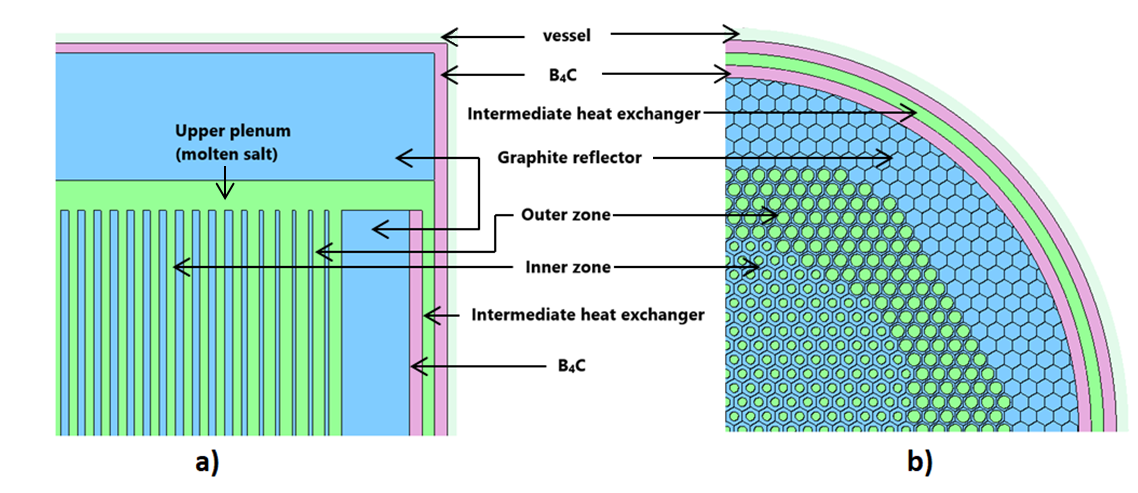
\includegraphics[width=\textwidth]{ff.png}
	\caption{$XZ$ (a) and $XY$ (b) section of the quarter-core model of the 
		SD-TMSR \cite{ashraf2019Preliminary}.}
	\label{fig:ff}
\end{figure}
In this study, the fuel salt composition is LiF-BeF$_2$-(HM)F$_N$ (70-17.5-12.5 mol\%),
where HM is the heavy metal (i.e., $^{232}$Th and fissile 
materials), and $N$ depends on the chosen fissile material and the 
thermochemical state of the liquid fuel salt. Three different types of initial 
fissile materials are considered: (1) $^{233}$U \cite{ashraf2020whole}, 
(2) reactor-grade Pu \cite{marka1993explosive}, and (3) transuranic (TRU) 
elements from \gls{LWR} \gls{SNF} \cite{de2000scenarios}.
The density and volume of the fuel salt are 3.3 g/cm$^{3}$ and 52.9 m$^3$, 
respectively. The liquid fuel salt circulates continuously through the channels
that pierce the graphite hexagonal prisms. The core is surrounded by 
axial and radial graphite reflectors to minimize the neutron leakage.
We adopted the same graphite density reported in the original SD-TMSR paper (2.3 g/cm$^3$) \cite{li_optimization_2018} to be consistent with results in the literature.
A 10-cm-thick B$_4$C cylinder surrounds the core to shield against neutrons and heat.
Finally, the SD-TMSR pressure vessel holds all reactor components and is made of 
a Hastelloy N alloy. The main characteristics of the SD-TMSR are 
summarized in Table~\ref{tab:table1}.


\begin{table}  %[!ht]
	\caption{The main characteristics of the SD-TMSR \cite{li_optimization_2018,ashraf2020whole}.}
	\vspace{0.1in}
	\begin{tabularx}{\textwidth}{l | r}
		\hline
		Thermal power, MW$_{th}$          				&  2,250  \\ 
		Fuel salt components                            & LiF-BeF$_2$-(\gls{HM})F$_N$ \\
		Fuel composition, mole\%                        & 70-17.5-12.5    \\
		$^7$Li enrichment, \%        				& 99.995   \\
		Fuel temperature, K 							& 900  \\
		Dilatation coefficient, g/(cm$^3$$\cdot{}$K)  &  -6.7$\times$10$^{-4}$ \\ 
		Fuel volume, m$^3$  &	52.9 \\
		Fuel density at 900 K, g/cm$^3$		  		& 3.3 \\
		Graphite density, g/cm$^3$             	    & 2.3	\\ 
		Core diameter, cm								& 460  \\
		Core height, cm									& 460  \\
		Side length of the graphite hexagonal prism, cm   & 7.5 \\
		Radius (inner fuel channel), cm							& 3.5  \\
		Radius (outer fuel channel), cm							& 5  \\
		Volume ratio of molten salt to graphite \\in the inner zone	&  0.357  \\
		Volume ratio of molten salt to graphite \\in the outer zone &  1.162  \\
		
		\hline
	\end{tabularx}
	\label{tab:table1}
\end{table}
%%%%%%%%%%%%%%%%%%%%%%%%%%%%%%%%%%%%%%%%

\subsection{Control rod design} \label{CRD}

The present paper proposes two sets of rods to control the reactivity of the SD-TMSR core:
\begin{enumerate}
\item Control Safety Devices (CSD);
\item Shutdown Safety Devices (SSD).
\end{enumerate}
The CSD system is designed for reactivity control during normal operation and the SSD system is designed for an emergency reactor shutdown.
In the present work, six different absorbing materials are considered based on their neutronics and safety performance:
\begin{enumerate}
\item natural B$_4$C (19.9\% $^{10}$B);
\item B$_4$C (enriched to 90\% $^{10}$B);
\item hafnium diboride (HfB$_2$);
\item hafnium hydride (HfH$_{1.62}$);
\item gadolinium oxide (Gd$_2$O$_3$);
\item europium oxide (Eu$_2$O$_3$).
\end{enumerate}

\begin{figure}[t!]  % replace 't' with 'b' to \centering
	\centering
	\hspace{+0.65in} 
	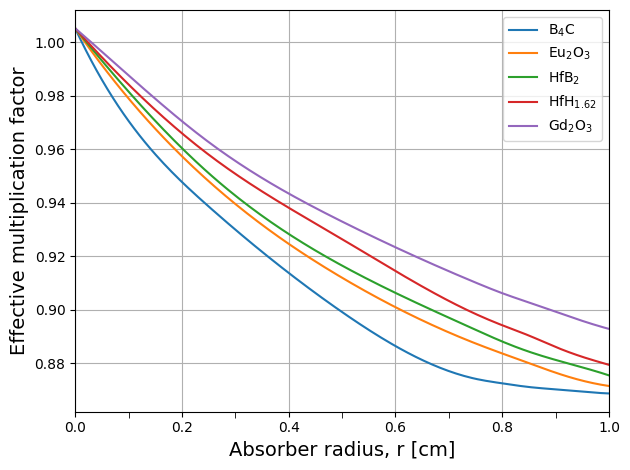
\includegraphics[width=\textwidth]{Radius.png}
	\caption{The change of the effective multiplication factor with the radius of the B$_4$C control rod.}
	\label{fig:Radius}
\end{figure}

The assessment of the optimal absorber radius should be an important consideration. If the CR radius is too large, the absorber material is not effectively utilized, due to self-shielding. We changed the radius of the CR and calculated the corresponding $k_{eff}$ when all CRs were fully inserted. Figure~\ref{fig:Radius} illustrates the change of the $k_{eff}$ with the radius of the B$_4$C control rod. As shown in Figure~\ref{fig:Radius}, in the region between 0 and 0.75 cm, the $k_{eff}$ decreases sharply with increasing absorber radius. However, in the region between 0.75 and 1.0 cm, there is almost no change in the $k_{eff}$. This is because of the geometry self-shielding of the neutron flux; beyond r = 0.75 cm, the $^{10}$B atoms in the central zone of the CR have relatively low chance for neutron capture.
From the obtained results, the control rod is a cylinder with a radius of 0.75 cm and a height of 520 cm. 
The absorbing material is surrounded by a 0.25-cm-thick cladding made of AIM1 
(15Cr-15Ni) steel alloy \cite{SERAN2017285} and the guide tube is made of 
SiC structural material (see Figure~\ref{fig:cr}). We simulated a 0.1-cm-thick gap between the 
cladding and guide tube to facilitate the control rod movement.
All densities of rod materials are listed in
Table~\ref{tab:table111}.

\begin{table}
	\caption{The densities of the absorbing materials.}
	\vspace{0.05in}
	\begin{center}	
		\begin{tabular}{l  r}  %[!ht]
			%%	\begin{tabularx}{\textwidth}{l | r}
			\hline
			Absorbers & Density [g/cm$^3$]\\
			\hline
			B$_4$C   &  2.54 \\
			HfB$_2$   &  10.5 \\
			HfH$_{1.62}$  &  11.4 \\
			Gd$_2$O$_3$   &  7.04 \\
			Eu$_2$O$_3$  &  7.38 \\
			SiC   & 3.21 \\
			AIM1 cladding   & 7.987 \\
			\hline
			%	\end{tabularx}
		\end{tabular}
		\label{tab:table111}
	\end{center}
\end{table}

%From the figure it can be seen that in the outer region of the B4C
%absorber, the flux is degraded rapidly, but in the region between 0 and 2 cm there is almost no change of the neutron flux. This phenomenon can be explained by the geometry self-shielding of the neutron flux. Due to absorption of low energy neutrons at the outside region ofthe absorber pin, the radius ofthe investigated pin is significantly larger than the penetration distance of the neutrons in the absorber. Therefore, the 10B atoms in the central part of the pin have no reasonable chance for neutron capture. Based
%
%
%On the basis of the obtained results the 5 ring configuration was selected for further
%ness (low self-shielding) and simplicity. On the basis of the obtained results the 5 ring configuration was selected for further
%analyses.
%
%This CR design consists of 61 absorber pins. Using Eq. (6) the radius of the absorber pins was calculated to 0.574 cm.
%
%In terms of neutronics, we an appropriate way to find the optimal pin radius could be the investigation of the neutron penetration distance, performed on a simple absorber pin.
%
%A single-pin design is a semi 1D approach preventing any interference caused by the self-shielding or geometrical influences of the surrounding absorber pins.

\begin{figure}[t!]  % replace 't' with 'b' to \centering
	\centering
	\hspace{+0.65in} 
	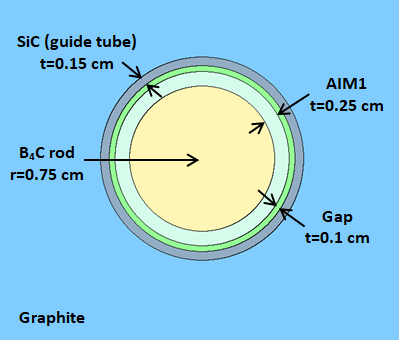
\includegraphics[width=\textwidth]{cr.png}
	\caption{Cross section of the B$_4$C control rod.}
	\label{fig:cr}
\end{figure}

Since the total number and distribution of the control assemblies in the SD-TMSR have not been determined, we propose an original distribution as a starting point of this analysis. We added clusters consisting of four control rods to specific graphite hexagonal prisms (elements) in the SD-TMSR core. Every four control rods can move together as one group (cluster). Figure~\ref{fig:graphite_elemen} demonstrates the plan view of the graphite element with the control rods. We propose 25 graphite elements with control rods: 16 Control Safety Devices (CSD) and 9 Shutdown Safety Devices (SSD).

\begin{figure}[t!]  % replace 't' with 'b' to \centering
	\centering
	\hspace{+0.65in}
	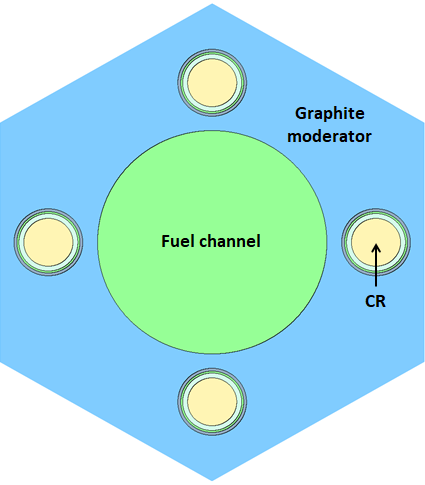
\includegraphics[width=\textwidth]{graphite_element.png}
	\caption{$XY$ section of graphite element with the four control rods 
	(cluster) located at the same distance from the fuel channel.}
	\label{fig:graphite_elemen}
\end{figure}
%\begin{figure}[t!]  % replace 't' with 'b' to \centering
%	\centering
%	\hspace{+0.65in}
%	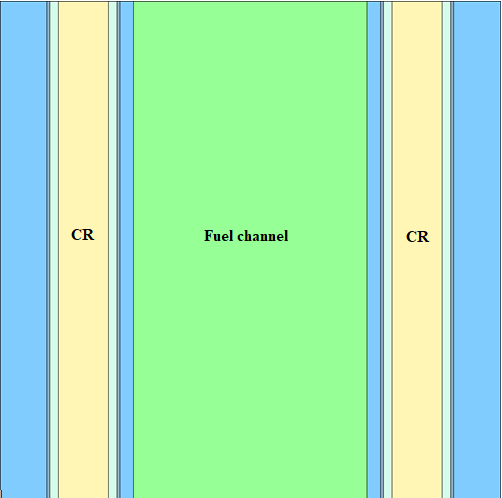
\includegraphics[width=\textwidth]{graphite_element1.png}
%	\caption{$XZ$ section of graphite element with control rods.}
%	\label{fig:graphite_elemen1}
%\end{figure}

Figure~\ref{fig:core_25} illustrates the numbering scheme of control rod 
clusters in the SD-TMSR core.
The CSD1-16 clusters are represented as yellow and distributed as two rings: inner and outer (peripheral) ring. The inner ring includes CSD from 1 to 6, while the outer ring includes CSD from 7 to 16. Red stands for SSD1-9 clusters.
We distributed the graphite elements with control rod clusters uniformly in 
the inner core of the SD-TMSR, in which the moderator-to-fuel ratio is high.
The selected core segment at the upper left corner of 
Figure~\ref{fig:core_25} shows that both CSD and SSD clusters consist of four 
control rods located at the same distance from the fuel channel center.
\begin{figure}[t!]  % replace 't' with 'b' to \centering
	\centering
	\hspace{+0.65in}
	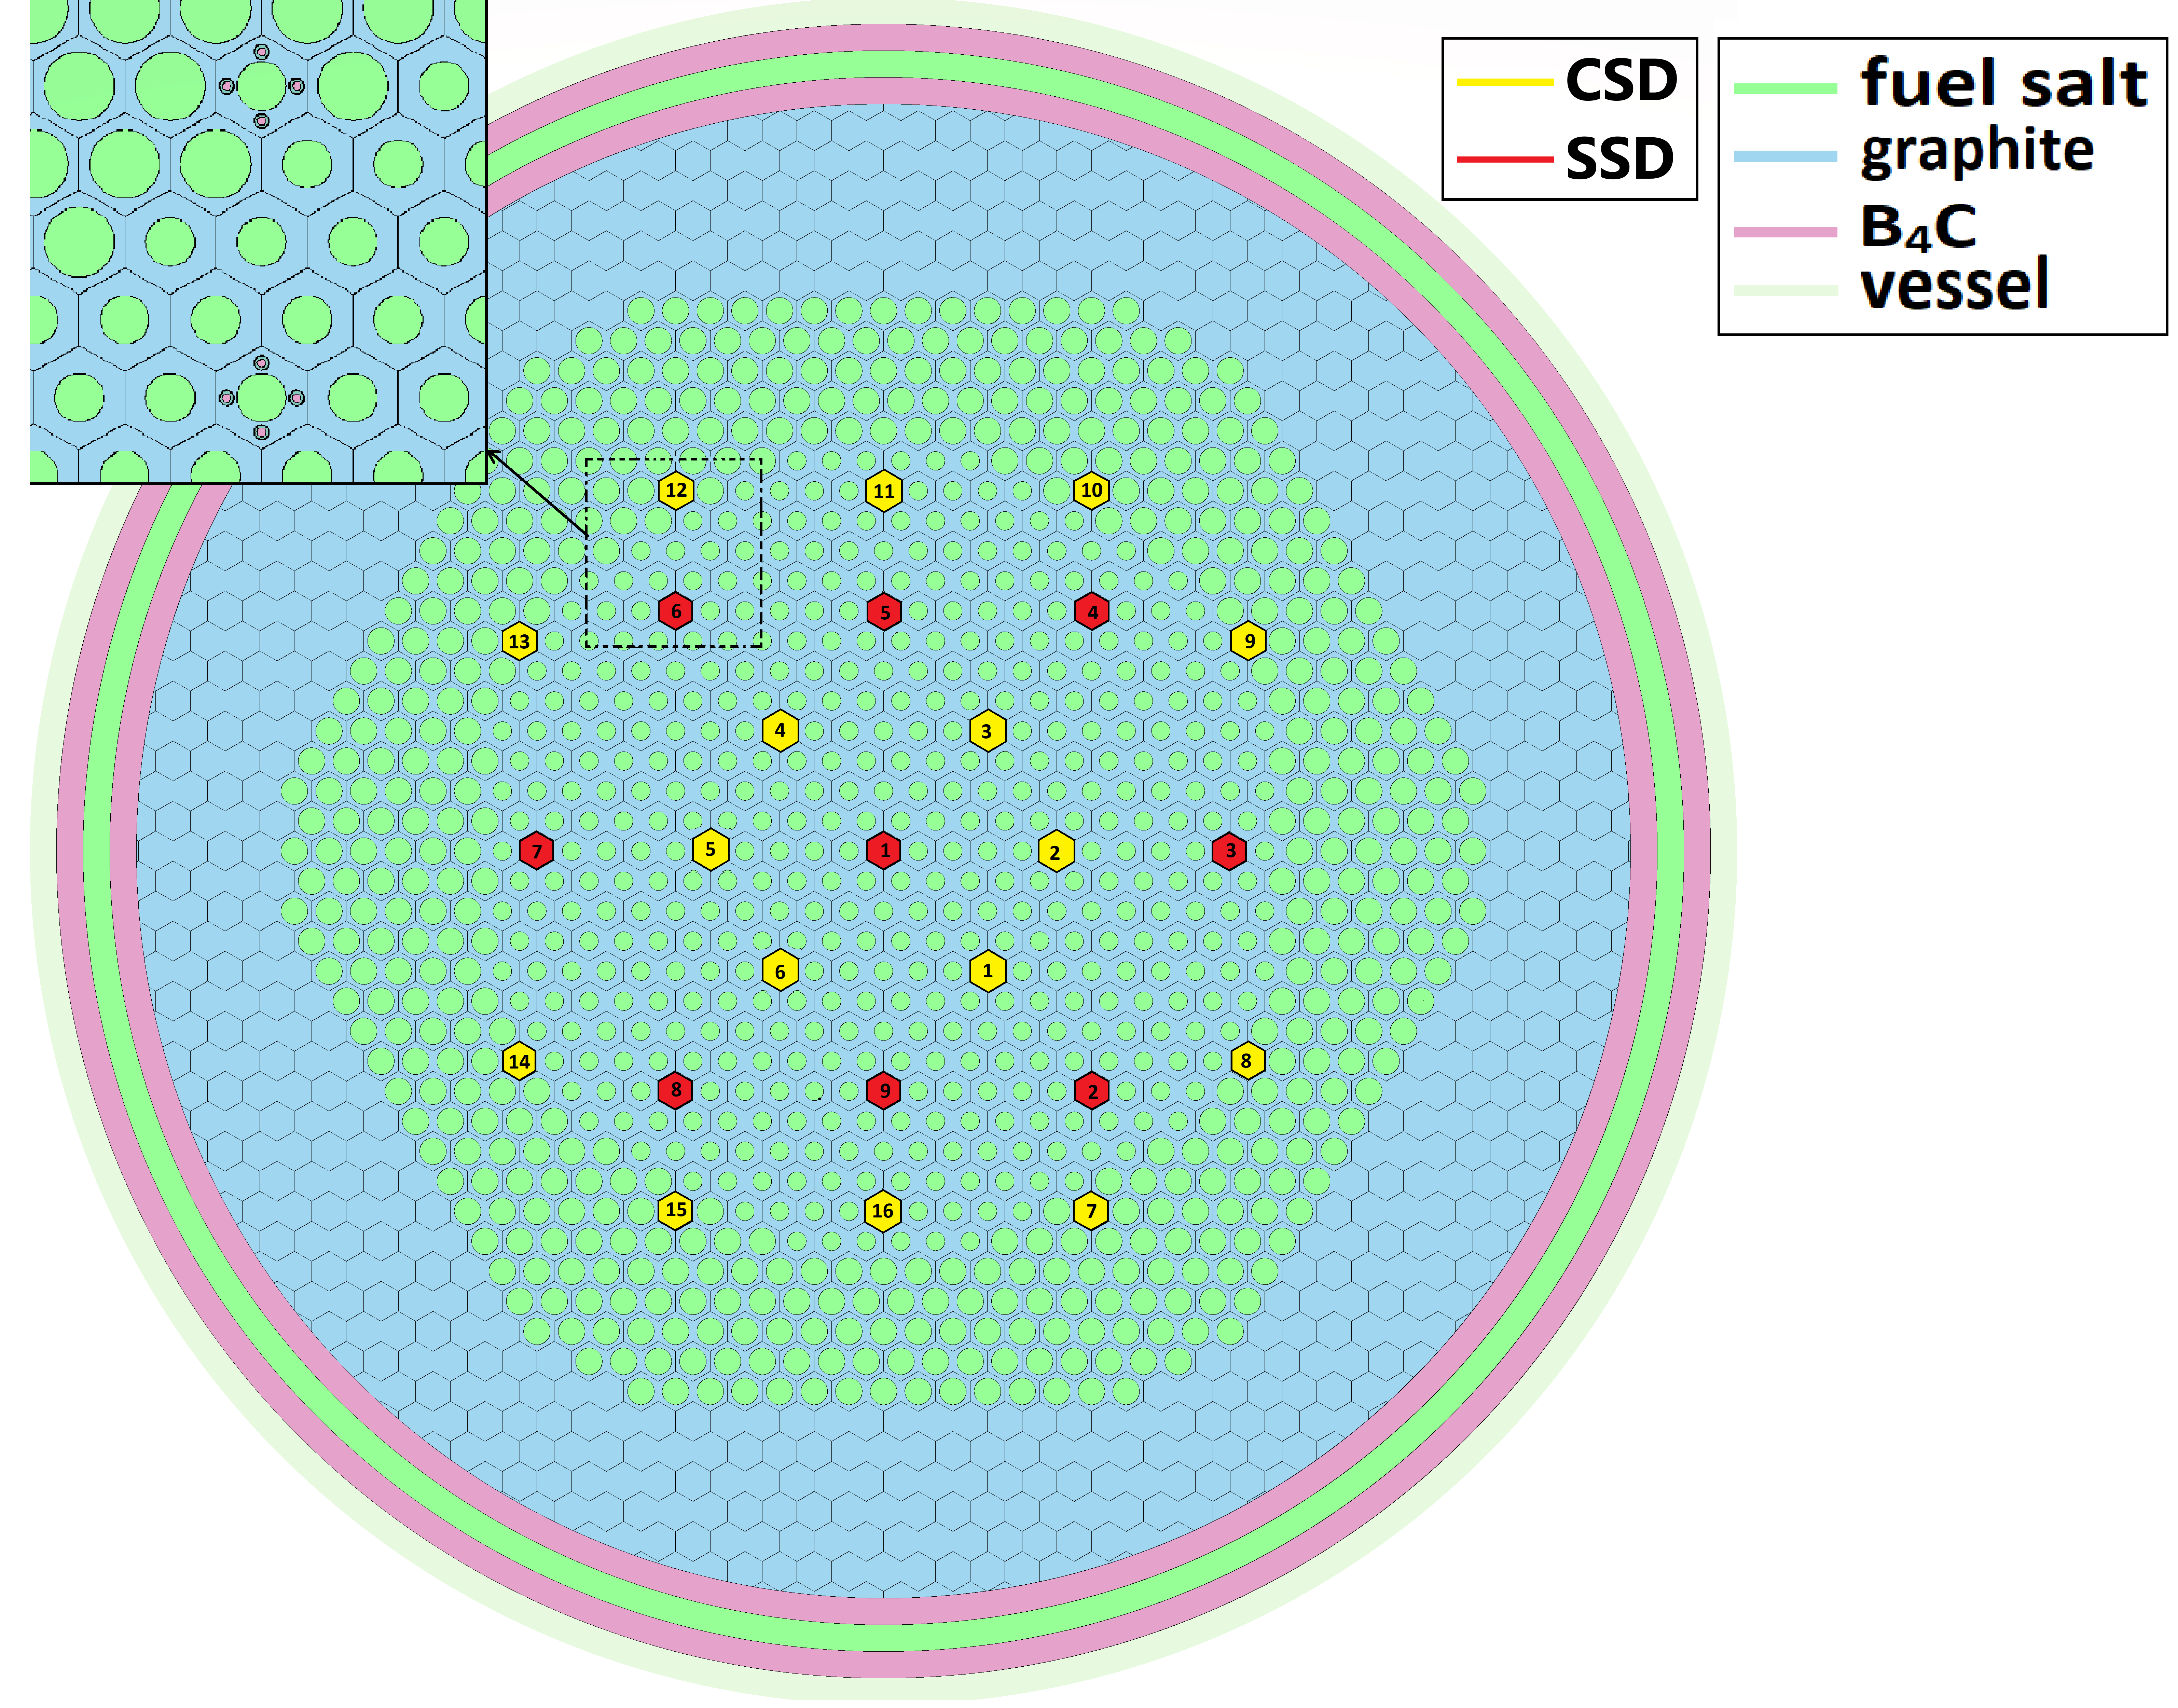
\includegraphics[width=\textwidth]{core_25.png}
	\caption{Distribution of the graphite elements with CRs in the SD-TMSR core.}
	\label{fig:core_25}
\end{figure}

\section{Methodology and tools} \label{Methodology-and-tools}
\subsection{Control rod design evaluation}
In this work, SERPENT-2 \cite{leppanen2014serpent} is used to 
perform steady-state calculations for a full 3D model of the SD-TMSR with 
the suggested control rod design. We adopted the ENDF-VII.0 cross section library 
for all calculations in the present work. The results demonstrated in this study were obtained after full-core calculations simulating 25$\times$10$^6$ active neutron histories per cycle. Simulations consisted in 500 active cycles of 5$\times$10$^4$ neutrons subdivided in 8 parallel tasks. Each simulation skipped 50 inactive cycles before beginning active tallies to allow for the convergence of the fission source distribution. Convergence has been checked through the fission source entropy. The statistical error in $k_{eff}$ was $\leq$ $25$ $pcm$.

%The results demonstrate whole-core runs of $50,000$ neutrons per cycle, for 50 inactive and 500 active cycles, and statistical error in $k_{eff}$ of $\leq$ $25$ $pcm$.
%
%Simulations consisted in 500 active cycles of 2∙104 neutrons. 20 inactive cycles were used for the convergence of the
%fission source distribution.
%
%Each simulation in this study skipped 200 generations before beginning active tallies to ensure fission source convergence.
%
%In order to minimize statistical errors and assure reliable fission source convergence, up to 2000 active fission source iteration cycles with 150,000 histories per cycle were used in neutron transport calculations with MCNP
%
%The MCNP transport step within the VESTA simulation uses 300 active cycles, 50 inactive cycles,
%and 100,000 particles per cycl
%
%The fission source defined in Serpent Code automatically dis-
%tributes the initial guess in fuel zones, with enhances the overall performance. Besides, the number of histories was selected to get the intended statistical convergence, considering the computa- tional effort involved. Accordingly, the following scheme was selected:
%? A Source with v3 ? 108 histories was selected for all cases where CRW is calculated in order to reach a statistical uncer- tainty of v5 pcm at 1 r for each calculation and a final value of CRW uncertainty below 5%.
%? A Source with v2 ? 107 histories was selected for all burnup cases in order to reach a statistical uncertainty of v20 pcm at 1 r for each calculation.
%3.3.
%
%The results presented in the following were obtained after full-core calculations simulating 250 million active neutron histories with the version 1.1.16 of the code. Simulations consisted in 500 active cycles of 5∙105 neutrons subdivided in 16 parallel tasks. Seventy inactive cycles were adopted to allow for the convergence of the fission source distribution. Convergence has been checked through the fission source entropy. Results

The initial calculation state of the SD-TMSR is identified by normal operation 
conditions (see Table~\ref{tab:table1}) and fully withdrawn control rod 
clusters. In this case, the control rods are located above the upper plenum as 
shown in Figure~\ref{fig:core_26}. To validate the proposed control rods 
system we adopted the same operation conditions (as in the initial calculation 
state) and changed the position of the control rod clusters along the $Z$ 
direction. The main calculated parameters including reactivity, control rod 
worth, and interference effects (shadowing effects) are described below.

\begin{figure}[t!] % replace 't' with 'b' to \centering
	\centering
	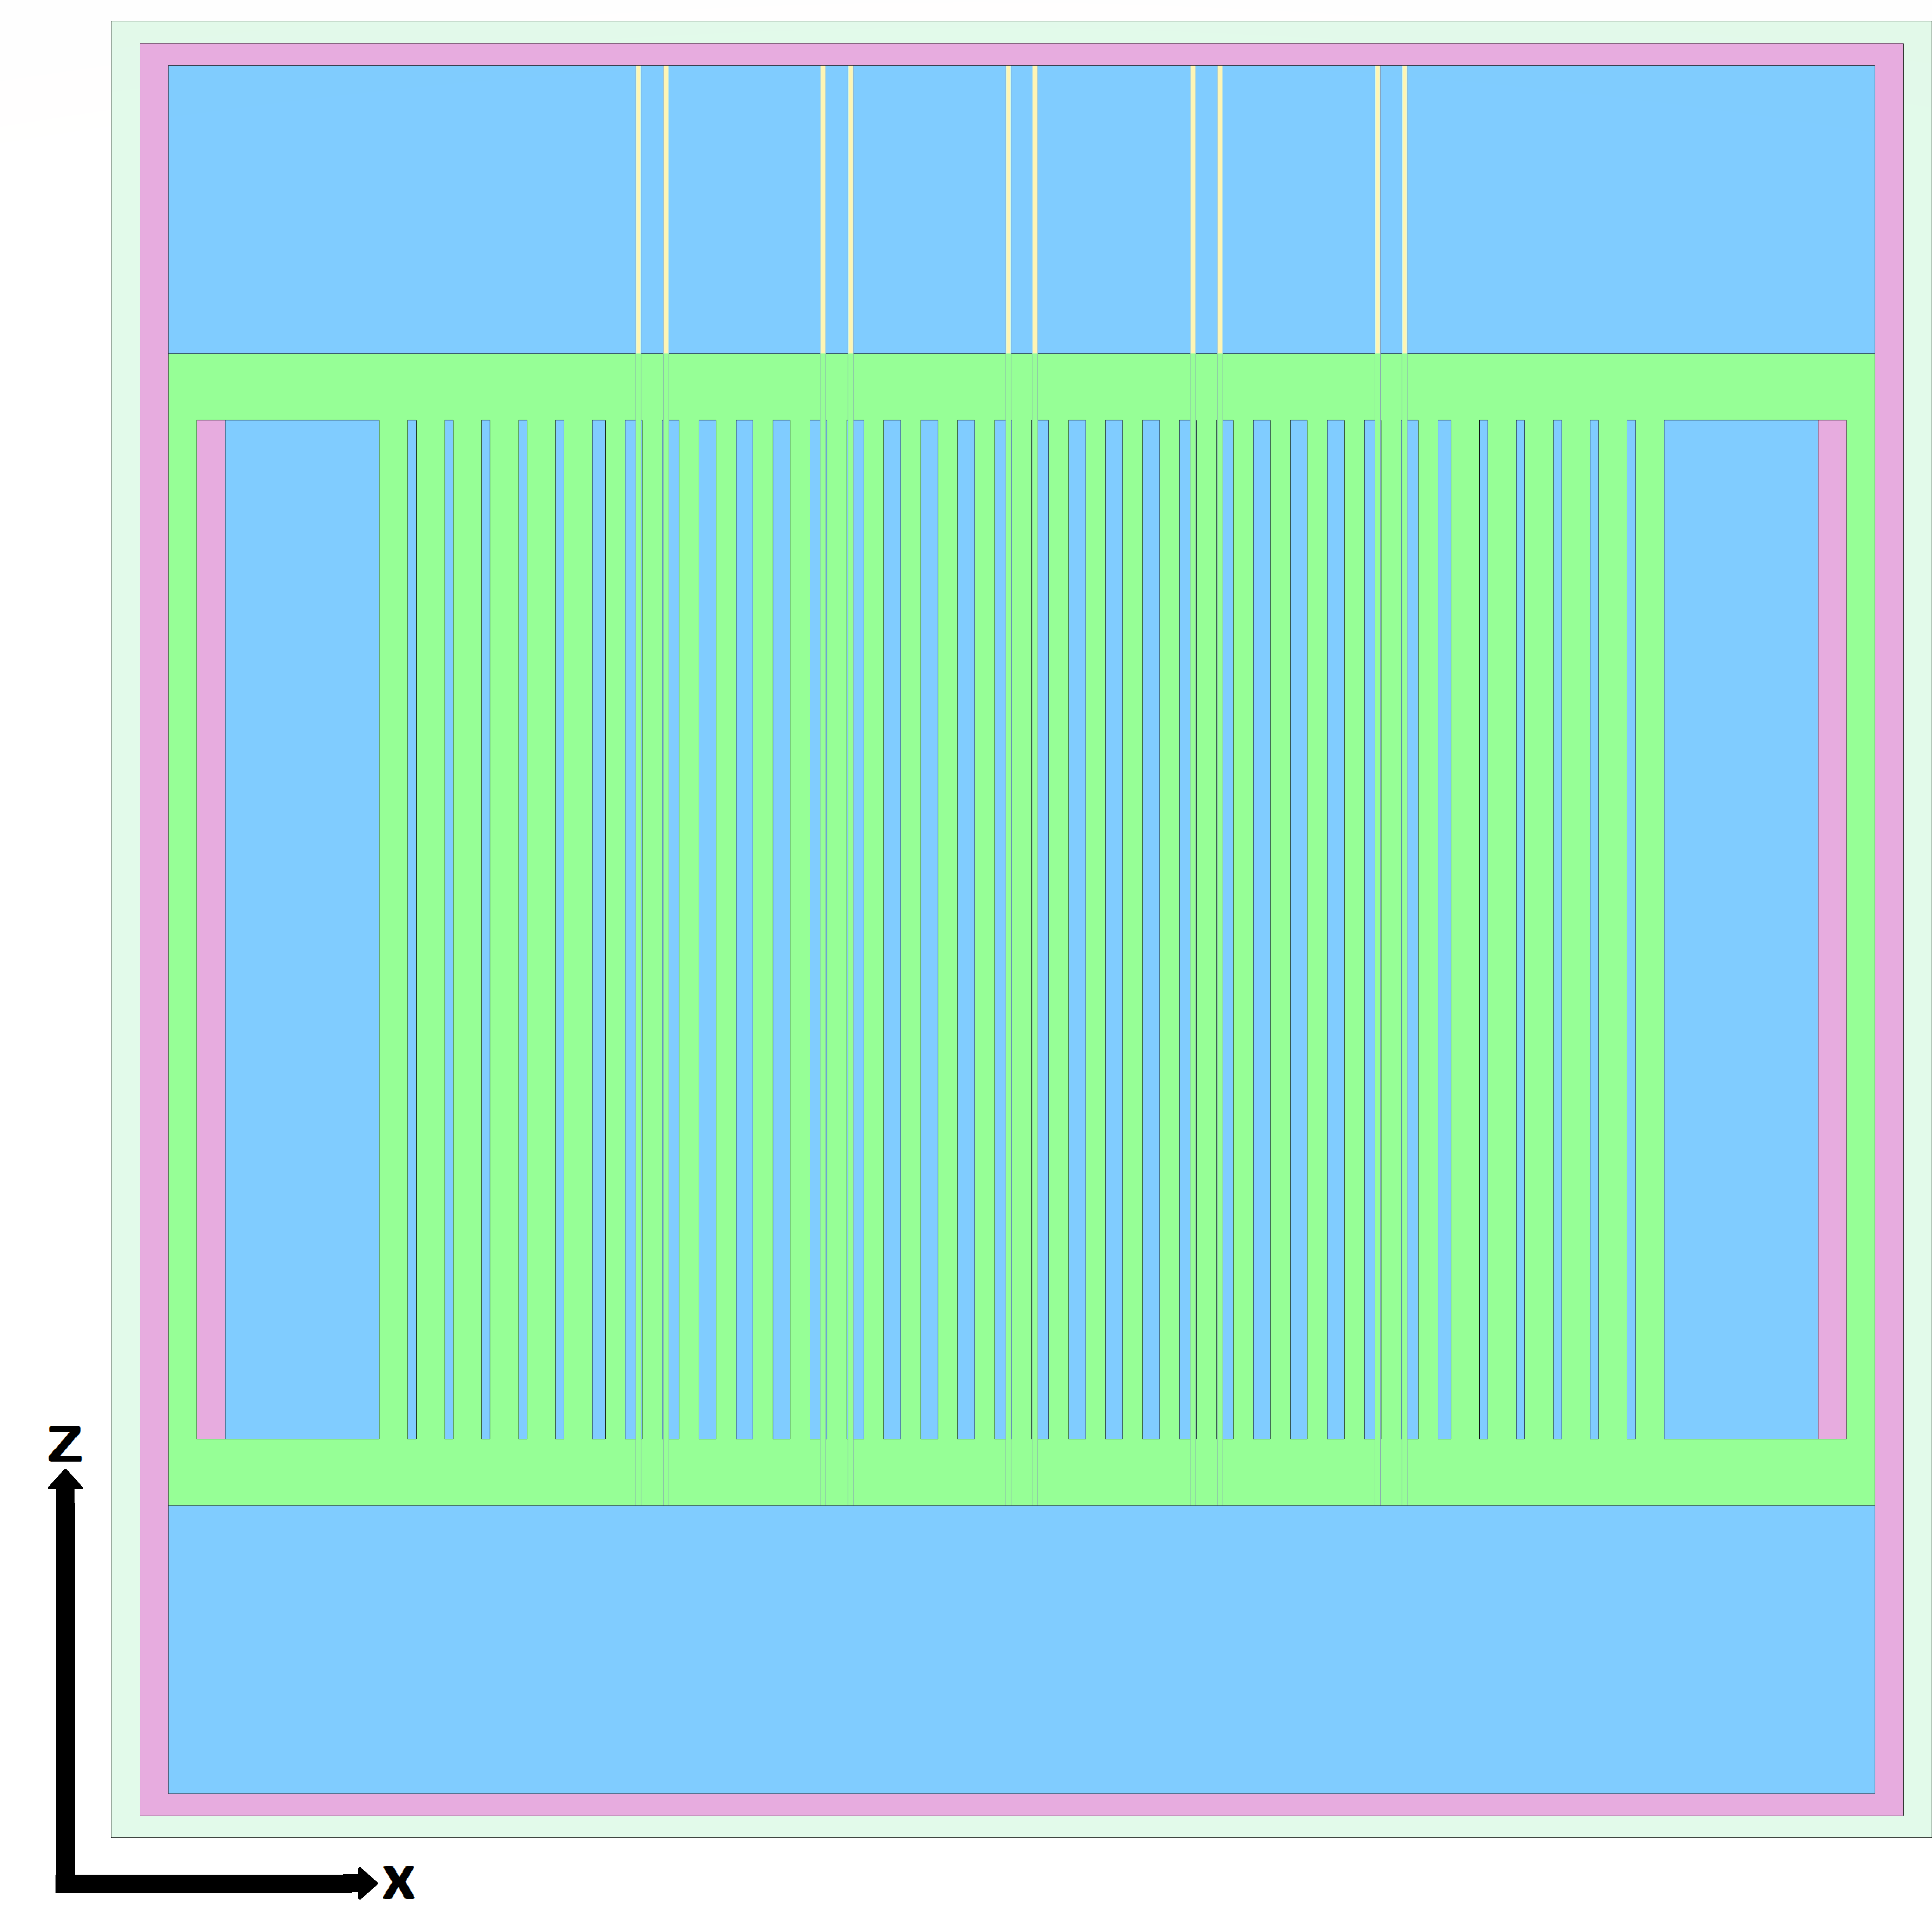
\includegraphics[width=\textwidth]{core_26.png}
	\caption{$XZ$ view at the midplane of the full-core model of the SD-TMSR, 10 CRs are fully withdrawn.}
	\label{fig:core_26}
\end{figure}

\subsubsection{Reactivity calculation}

The excess reactivity $\rho$$_e$ is the reactivity of the core when all control rods are withdrawn. $\rho$$_e$ is calculated by SERPENT-2 in \$ units based on equation~\ref{Equ:1}, where $k_{eff}$ is the effective multiplication factor of the core and $\beta_{eff}$ is the effective fraction of delayed neutrons:

\begin{equation}
\label{Equ:1}
{{\rho}_{e}}=\dfrac{{k_{eff}}-1}{{k_{eff}}{{\beta}_{eff}}}.
\end{equation}

The effective delayed neutron fraction is calculated by the adjoint-weighted time constants using a perturbation technique in SERPENT-2 \cite{leppanen2014calculation} and it accounts for the steady-state of the fuel salt.

\subsubsection{The control rod worth (CRW)}

The control rod worth (CRW) is the amount of negative reactivity associated with the control rod insertion. The CRW is calculated by SERPENT-2 in \$ units based on equation~\ref{Equ:2}, where $\Delta\rho$$_{CRi}$ is the worth of the i$^{th}$ control rod (CR), $\rho$$_e$ is the initial excess reactivity, and $\rho$$_{CRi}$ is the excess reactivity after insertion of the i$^{th}$ CR \cite{vcerba2017optimization}:

\begin{equation}
\label{Equ:2}
{{\Delta}{\rho}_{CRi}}={{\rho}_{e}}-{{\rho}_{CRi}}.
\end{equation}

\subsubsection{Shutdown margin (SDM)}

The shutdown margin (SDM) is the amount of reactivity by which a full reactor core is subcritical from a given state. The Shutdown Safety Devices (SSD) clusters are designed mainly for an emergency shutdown, thus it should 
provide the reactor core with sufficient negative reactivity. The SDM is expressed in terms of reactivity and calculated by equation~\ref{Equ:6}, where $\Delta\rho_{SSD}$ is the total worth of the Shutdown Safety Devices (SSD) and $\rho$$_e$ is the core excess reactivity:

\begin{equation}
\label{Equ:6}
{SDM}={{\Delta}{\rho}_{SSD}}-{{\rho}_{e}}.
\end{equation}

\subsubsection{Interference effects (shadowing effects)}

Interference between control rods (CRs) or shadowing effects occur when one 
(or more) control rod impacts the reactivity worth of another control rod in 
the surroundings. 
The insertion of a CR depresses the neutron flux
in its vicinity and makes the curvature of the neutron flux greater. The gradient
of the neutron flux will contrarily increase at a radial distance. The CRs, distributed in the core,
will distort the neutron flux around each other and will impact the reactivity worth.
The term ``shadowing effect" has been used to describe this \cite{oka2014nuclear}.
The shadowing effect appears when the combined rod worth
is less than the sum of the individual worths. Meanwhile, anti-shadowing is observed 
when the combined rod worth is greater than the sum of the individual worths.
The core height-to-diameter ratio (H/D), CR locations, and the three-dimensional configuration 
of the CRs affect the degree of the interference between CRs \cite{oka2014nuclear}. 

The amplification factor of the i$^{th}$ CR (A$_{CRi}$) helps to evaluate the shadowing effects between CR clusters. The A$_{CRi}$ is calculated by equation~\ref{Equ:3} \cite{vcerba2017optimization}, where $\Delta\rho$$_{CR(1,2,\ldots N)}$ is the total worth of all CRs (from $1$ to $N$), $\Delta\rho$$_{CR(1,2,\ldots N-i)}$ is the total worth of all CRs except the i$^{th}$ rod, and $\Delta\rho$$_{CRi}$ is the worth of the i$^{th}$ rod:

\begin{equation}
\label{Equ:3}
{{A}_{CRi}}=\dfrac{{{\Delta}{\rho}_{CR(1,2,\ldots N)}}-{{\Delta}{\rho}_{CR(1,2,\ldots N-i)}}}{{\Delta}{\rho}_{CRi}}.
\end{equation}

If A$_{CRi}$ is $<$1, the CRW is reduced due to shadowing effects, but if A$_{CRi}$ is $>$1, the CRW is amplified and anti-shadowing effects occur \cite{girardin2007control}. A$_{CRi}$ = 1 means no shadowing effects occur.

\subsubsection{Integral and differential control rod worth}

The integral CRW is the total reactivity change due to the full 
insertion or withdrawal of the CR. However, the \textit{differential CRW} is the
reactivity inserted per unit of withdrawal [\$/cm]. To calculate those 
parameters, we varied the position of CR clusters from fully withdrawn to 
fully inserted. Equation~\ref{Equ:4} is used to calculate the integral CRW 
[\$], where $k_{j-1}$ and $k_{j}$ are the effective multiplication factors 
before and after CR insertion to the $j$$^{th}$ step, respectively, $\beta_{j}$ is the
fraction of delayed neutrons at the $j$$^{th}$ step, and $N$ is the number of steps:

\begin{equation}
\label{Equ:4}
{{\Delta}{\rho}_{j}}=\sum_{j=1}^{N}\dfrac{{k_{j}}-{k_{j-1}}}{{{k_{j}}{k_{j-1}}}{{\beta}_{j}}}.
\end{equation}

Equation~\ref{Equ:5} is used to calculate the theoretical differential CRW, where 
$\Delta Z$ is the length of rod inserted:

\begin{equation}
\label{Equ:5}
\dfrac{{\partial}{\rho}_{j}}{{\partial{Z}}}=\dfrac{1}{{\Delta}{Z}}\dfrac{{k_{j}}-{k_{j-1}}}{{{k_{j}}{k_{j-1}}}{{\beta}_{j}}}.
\end{equation}


